\documentclass[a4paper,9pt,twoside]{report}

\usepackage[margin=1.2cm]{geometry}
\usepackage{amsmath}
\usepackage{titling}
\usepackage{fontspec}
\usepackage{listings}
\usepackage{hyperref}
\usepackage{graphicx}
\usepackage{float}

\usepackage[dutch]{babel}

\usepackage{fontspec}
\setmainfont{Montserrat}

\usepackage{titlesec}

\titleformat{\chapter}[display]{\normalfont\bfseries}{}{0pt}{\Huge}

\title{Nieuwsartikel}

\author{Dylan {Cluyse}}

\begin{document}
	
\chapter{Hoe \textit{Pentimentor} jou kan helpen bij het begrijpend lezen}

\noindent Plaats jezelf in de schoenen van een scholier met dyslexie in de derde graad van het middelbaar onderwijs. Voor een opdracht begrijpend lezen moet jij het volgende deel uit een wetenschappelijk artikel doornemen, afgebeeld op onderstaande simulatie.

\begin{figure}[H]
	\fbox{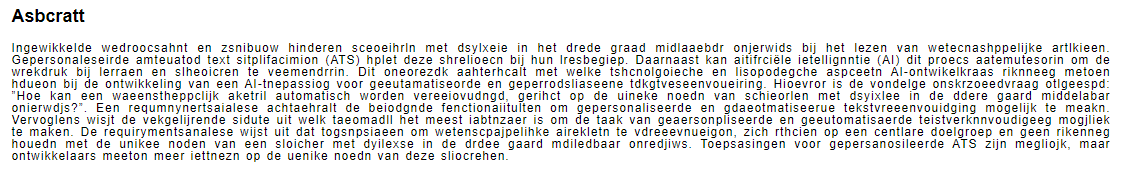
\includegraphics[width=\linewidth]{1-screenshot-abstract.png}}	
\end{figure}

\noindent Moeilijker dan je denkt? Onderschat de uitdaging niet! Hoewel symptomen van dyslexie niet alleen 'dansende letters'  zijn, toont deze simulatie dat dit één van de obstakels is die dyslectische scholieren kunnen ervaren. Leerkrachten zouden de oorspronkelijke tekst in een andere lay-out kunnen gieten. Zo kunnen aangepaste lettertypes, woordspatiëring of regelafstand het lezen van een artikel aangenamer maken voor een scholier met dyslexie.

\medspace

\noindent Bovendien vereist het lezen van wetenschappelijke artikelen specifieke vakkennis. Deze artikelen kunnen scholieren in de derde graad van het middelbaar onderwijs sterker motiveren om hun opleiding verder te zetten in het hoger onderwijs. Het begrijpen van tekstinhoud kan echter een lastige taak zijn. De oplossing hiervoor: tekstvereenvoudiging. Door de woordenschat en zinsbouw aan te passen, maken auteurs deze artikelen opnieuw toegankelijk voor een lager wetenschappelijk geletterde doelgroep. 

\subsubsection{De uitdaging met tekstvereenvoudiging}

\noindent Personaliseerbare tekstvereenvoudiging heeft een bewezen effect op het leereffect van scholieren in het middelbaar onderwijs, maar dit proces vraagt tijd en energie van de auteur.

\medspace

\noindent Tekstvereenvoudigingstoepassingen bestaan al, maar ze ontbreken de nodige personaliseerbaarheid en veranderen de moeilijkheidsgraad van de oorspronkelijke tekst niet. Daarnaast beschikken software-ontwikkelaars over onvoldoende logopedische voorkennis om deze toepassingen te ontwikkelen. Bovendien kan dergelijke toepassing iedereen in het onderwijs baten. Om te bewijzen dat ontwikkelaars hier wél met de huidige middelen toe in staat zijn, ontwikkelde dit onderzoek een prototype: \textit{Pentimentor}.

\subsubsection{\textit{Pentimentor}: Het nieuwste van het nieuwste.}

\textit{Pentimentor} is een tool om pdf-documenten te vereenvoudigen en samen te vatten. Allereerst kan je op een aanpasbare webpagina het oorspronkelijke wetenschappelijke artikel lezen. In deze omgeving kan je delen tekst in het artikel markeren, zodat je deze vervolgens kan laten vereenvoudigen of samenvatten door \textit{Pentimentor}. Daarnaast kan je ook specifieke vragen stellen over de inhoud van de gemarkeerde tekst. Tot slot biedt \textit{Pentimentor} de mogelijkheid om een nieuw Word-document te genereren met daarin de vereenvoudigde tekst.

\medspace

\noindent Om tekstaanpassingen in deze mate mogelijk te maken, gebruikt \textit{Pentimentor} het GPT-3 model. Als die naam je bekend in de oren klinkt, dan is dat geen toeval, want dit is het achterliggende taalmodel van ChatGPT. Maar waarom specifiek dit taalmodel? GPT-3 kan personaliseerbare uitvoer genereren. Afhankelijk van jouw keuzes kan het vereenvoudigde document anders zijn dan dat van andere gebruikers.

\medspace

\noindent Het is mogelijk om voor de lezer ongekende woorden mee te geven. Nadien vereenvoudigt het taalmodel, wat niet mogelijk is bij andere toepassingen op de markt. Dit prototype probeert de achtergrondkennis van de eindgebruiker goed in te schatten. Daarmee laat het prototype geen gekende kennis achterwege en kan het een merkbaar leereffect aanreiken.

\subsubsection{\textit{Keep it simple, stupid}}

\noindent Ontwikkelaars maken graag indruk met hun toepassingen. Bestaande toepassingen die teksten kunnen samenvatten of vereenvoudigen, zijn overladen met functies, waardoor gebruikers het overzicht kwijtraken. Daarom richt \textit{Pentimentor} zich op eenvoud. Hier kunnen gebruikers kiezen hoe het systeem de wetenschappelijke inhoud weergeeft of verandert, op manieren die andere systemen niet kunnen. Hierdoor maakt het prototype alle voorgaande toepassingen overbodig. Zo toont de onderstaande afbeelding hoe \textit{Pentimentor} op een eenduidige manier ondersteuning aan scholieren kan bieden.

\begin{figure}[H]
	\fbox{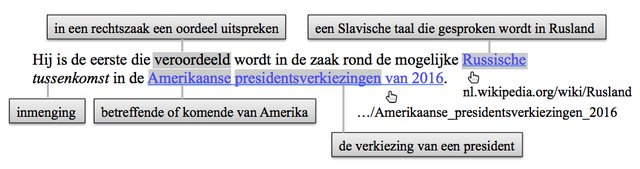
\includegraphics[width=\linewidth]{dutch-simplification-dyslexia-example.png}}
\end{figure}
	
\subsubsection{\textit{Pentimentor} vergeleken met de uitgeteste tools}

Uit een vergelijkende studie blijkt dat \textit{Pentimentor} duidelijk boven andere tools staat. Zo ontbreekt personaliseerbaarheid in de uitgeteste tools. De uitvoer is identiek bij iedere eindgebruiker. Daarnaast kunnen deze tools geen wetenschappelijke concepten samenvatten in een overzichtelijke vorm, zoals een tabel.

\medspace

\noindent De presentatie van het artikel is enkel een bijzaak bij de andere tools. \textit{Pentimentor} houdt hier wel rekening mee door het oorspronkelijke en het vereenvoudigde artikel op één personaliseerbare pagina te tonen. Dit speelt een rol bij scholieren met leesstoornissen, waaronder dyslexie. Geen enkele toepassing is in staat om een Word-document te maken, terwijl \textit{Pentimentor} dit wel kan. Zo kan de eindgebruiker nog zaken, zoals lay-out, aanpassen indien nodig.

\medspace

\noindent Ten slotte kan \textit{Pentimentor} duidelijk de link met het oorspronkelijke artikel leggen. Andere toepassingen doen dit niet en verwachten dat de eindgebruiker deze zelf kan leggen. Bij dergelijke toepassingen ligt de focus te weinig op de relatie tussen de oorspronkelijke en aangepaste tekst. \textit{Pentimentor} zet ontwikkelaars hiertoe aan.

\subsubsection{Tot slot}

\noindent Is \textit{Pentimentor} de ultieme oplossing? Nog niet. 

\medspace

\noindent Hoewel \textit{Pentimentor} veelbelovende teksten kan schrijven, bevindt het zich nog in de prototypefase en vereist het verdere ontwikkeling. Software-ontwikkelaars beschikken wel degelijk over de nodige middelen om het concept concreet uit te werken. Zo kunnen zij teksten laten herschrijven met het GPT-3 taalmodel zonder dat ze zelf een taalmodel moeten ontwikkelen. Als je \textit{Pentimentor} zelf wil uittesten, kan je het downloaden en installeren volgens de instructies op deze link.

\end{document}